\chapter{Bildanhänge}

\begin{figure}[h!]
    \centering
    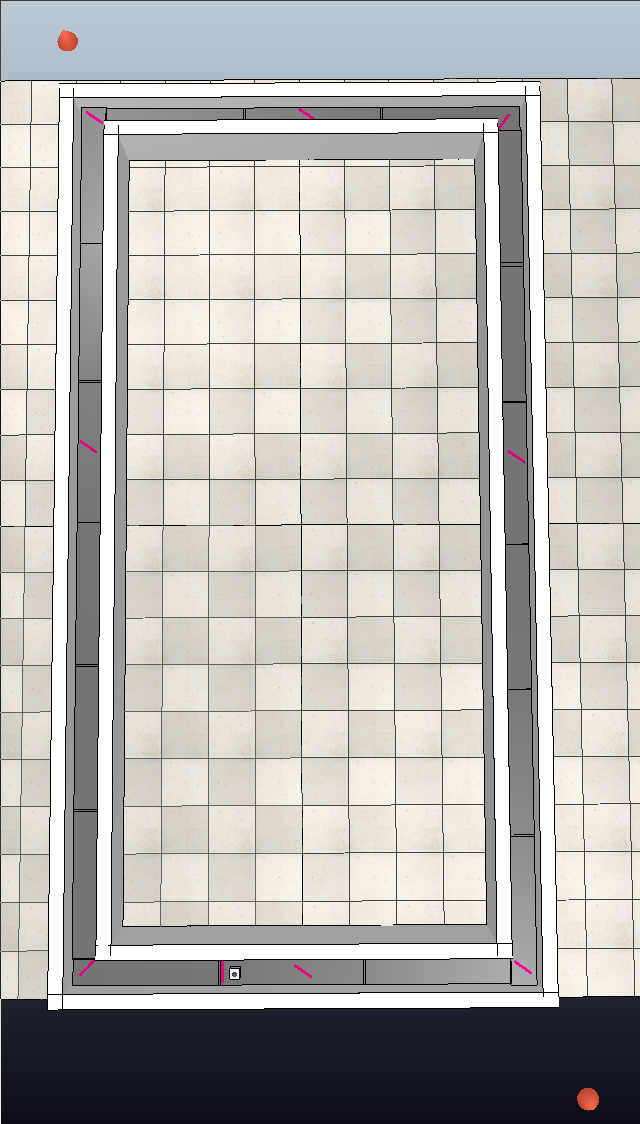
\includegraphics[angle=90, width=\linewidth]{images/long_rectangle.png}
    \caption{Modell der Route \glqq long\_rectangle\grqq\ in CoppeliaSim.}
    \label{fig:long_rectangle}
\end{figure}

\begin{figure}[h!]
    \centering
    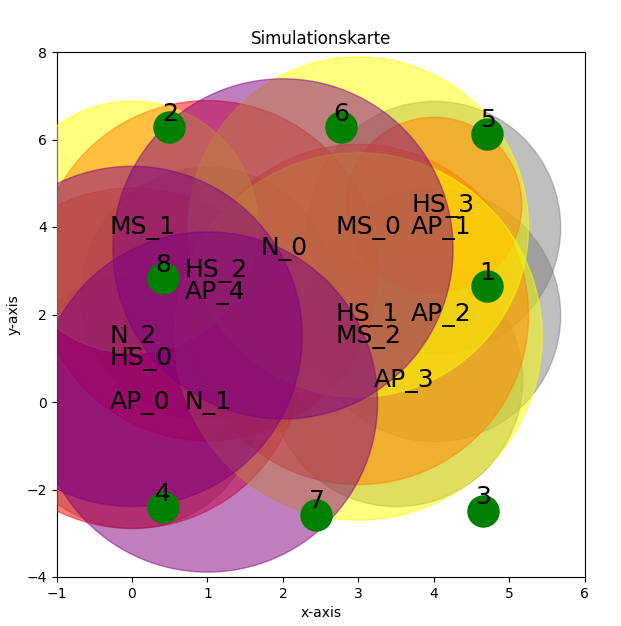
\includegraphics[width=0.9\linewidth]{images/long_rectangle_simulation_map.png}
    \caption{Karte der Route \glqq long\_rectangle\grqq\ mit eingezeichneten Einflussbereichen der Objekte, die Einfluss auf modellierte Sensoren haben.
    \textit{\textbf{M}agnetic \textbf{S}ource} (Gelb), \textit{\textbf{N}oise Source} (Lila), \textit{\textbf{A}ccess \textbf{P}oint} (Grau),
    \textit{\textbf{H}eat \textbf{S}ource} (Rot) und Standorte (Grün).}
    \label{fig:long_rectangle_simulation_map}
\end{figure}

\begin{figure}[h!]
    \centering
    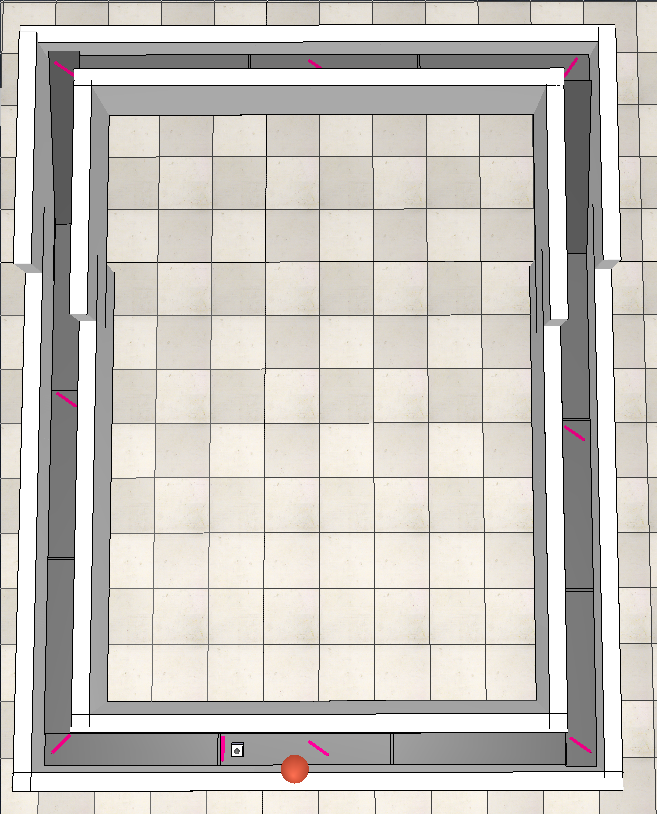
\includegraphics[angle=90, width=\linewidth]{images/rectangle_with_ramp.png}
    \caption{Modell der Route \glqq rectangle\_with\_ramp\grqq\ in CoppeliaSim.}
    \label{fig:rectangle_with_ramp}
\end{figure}

\begin{figure}[h!]
    \centering
    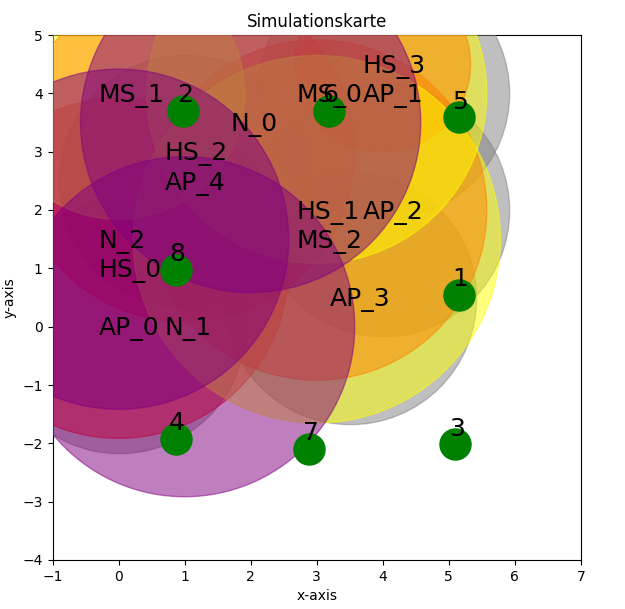
\includegraphics[width=0.9\linewidth]{images/rectangle_with_ramp_simulation_map.png}
    \caption{Karte der Route \glqq rectangle\_with\_ramp\grqq\ mit eingezeichneten Einflussbereichen der Objekte, die Einfluss auf modellierte Sensoren haben.
    \textit{\textbf{M}agnetic \textbf{S}ource} (Gelb), \textit{\textbf{N}oise Source} (Lila), \textit{\textbf{A}ccess \textbf{P}oint} (Grau),
    \textit{\textbf{H}eat \textbf{S}ource} (Rot) und Standorte (Grün).}
    \label{fig:rectangle_with_ramp_simulation_map}
\end{figure}

\begin{figure}[h!]
    \centering
    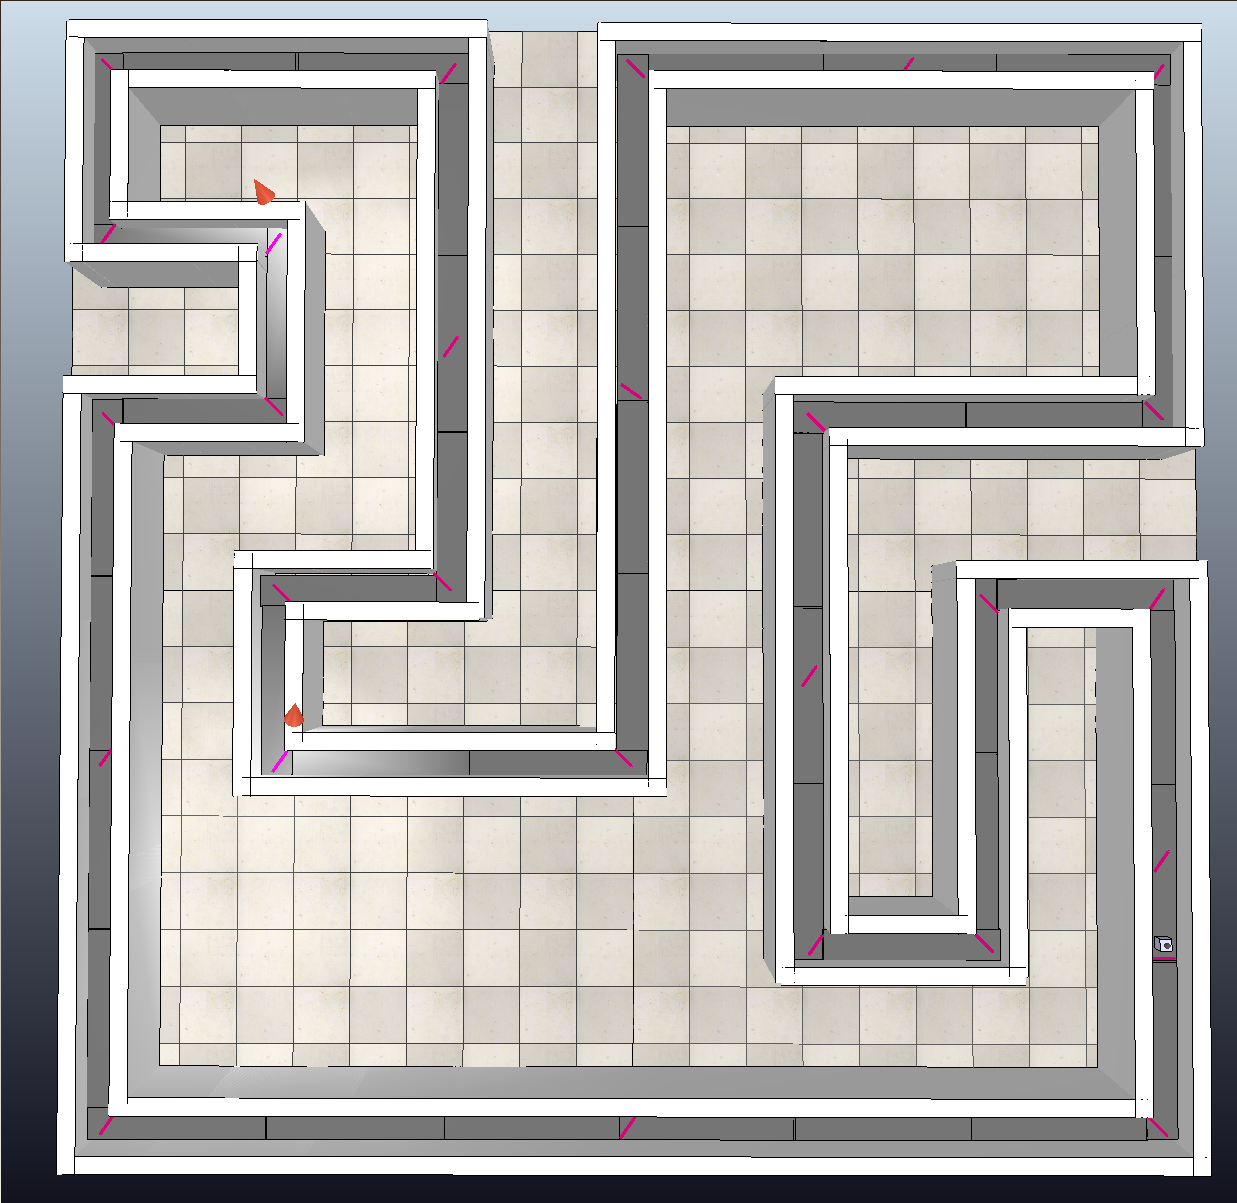
\includegraphics[width=\linewidth]{images/many_corners.png}
    \caption{Modell der Route \glqq many\_corners\grqq\ in CoppeliaSim.}
    \label{fig:many_corners}
\end{figure}

\begin{figure}[h!]
    \centering
    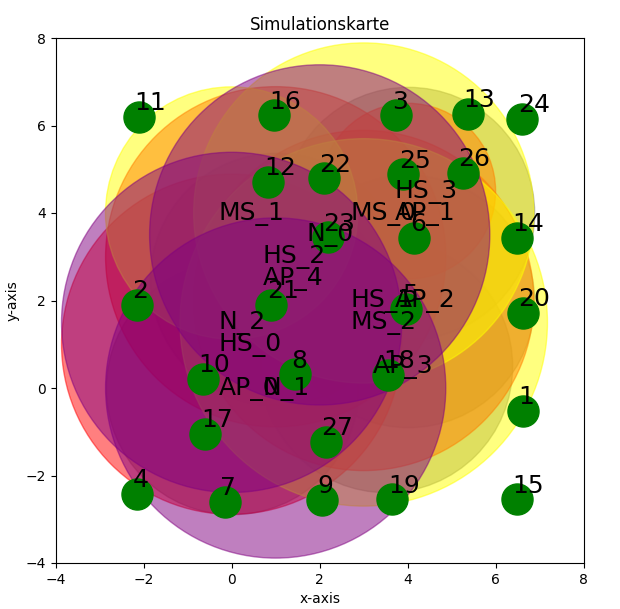
\includegraphics[width=0.9\linewidth]{images/many_corners_simulation_map.png}
    \caption{Karte der Route \glqq many\_corners\grqq\ mit eingezeichneten Einflussbereichen der Objekte, die Einfluss auf modellierte Sensoren haben.
    \textit{\textbf{M}agnetic \textbf{S}ource} (Gelb), \textit{\textbf{N}oise Source} (Lila), \textit{\textbf{A}ccess \textbf{P}oint} (Grau),
    \textit{\textbf{H}eat \textbf{S}ource} (Rot) und Standorte (Grün).}
    \label{fig:many_corners_simulation_map}
\end{figure}

\begin{figure}[h!]
    \centering
    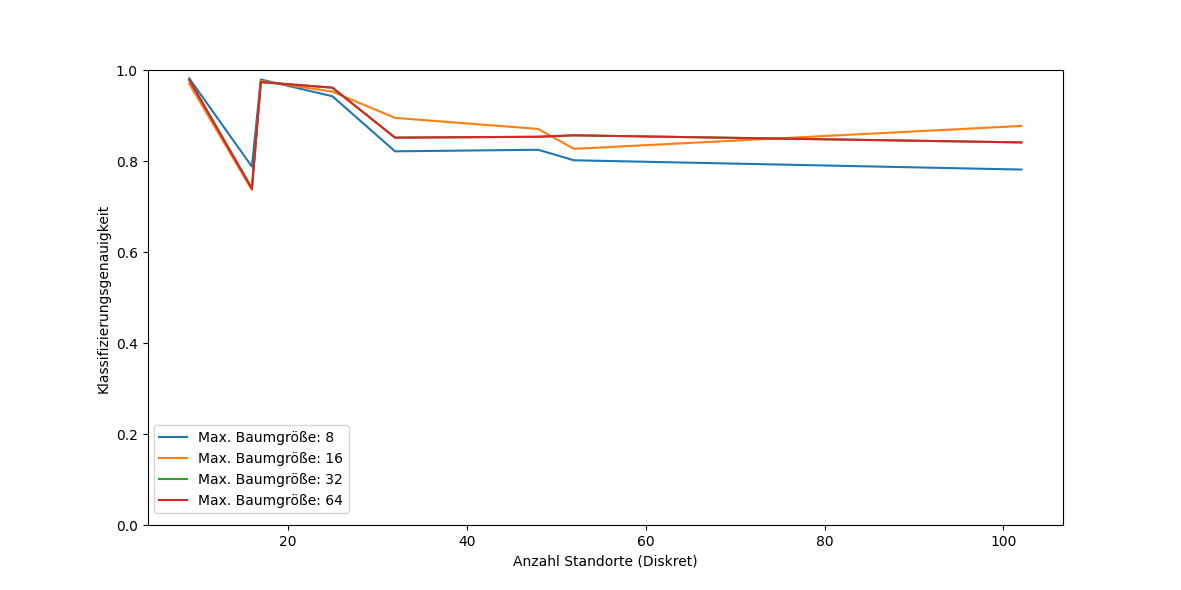
\includegraphics[width=\linewidth]{images/multiple_best_by_group_dt_max_depth_acc_5_cont.png}
    \caption{Klassifizierungsgenauigkeiten $P(B\leq5)_{\text{cont}}$ von Entscheidungswäldern mit einer Waldgröße von 16 über Standortkomplexitäten.}
    \label{fig:multiple_best_by_group_dt_max_depth_acc_5_cont}
\end{figure}

\begin{figure}[h!]
    \centering
    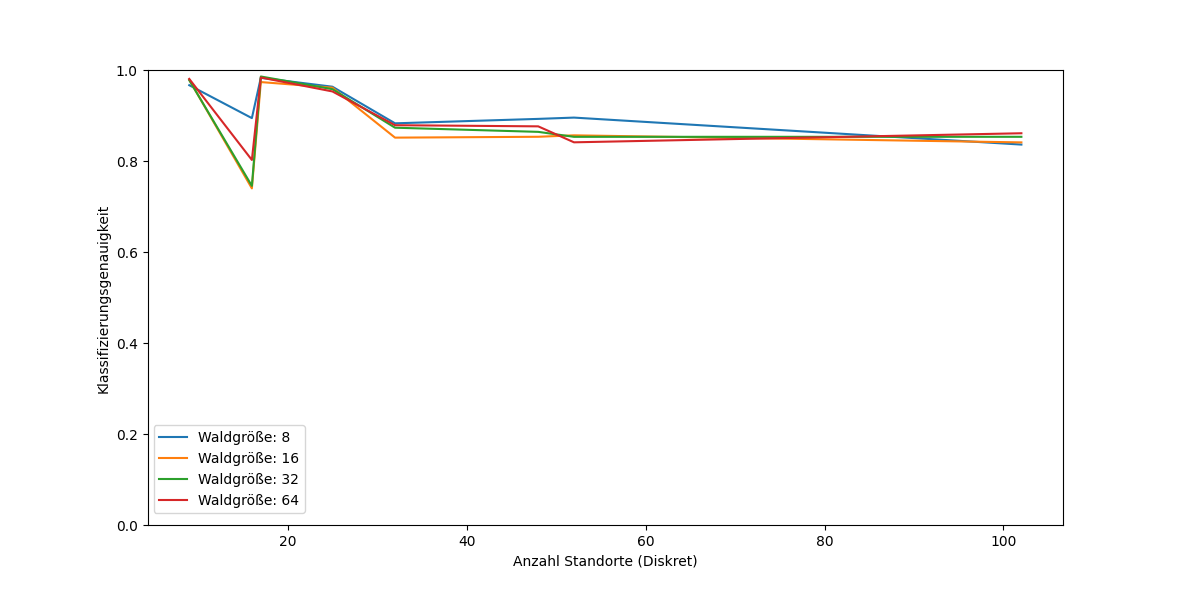
\includegraphics[width=\linewidth]{images/multiple_best_by_group_dt_trees_acc_5_cont.png}
    \caption{Klassifizierungsgenauigkeiten $P(B\leq5)_{\text{cont}}$ von Entscheidungswäldern mit einer maximalen Baumhöhe von 32 über Standortkomplexitäten.}
    \label{fig:multiple_best_by_group_dt_trees_acc_5_cont}
\end{figure}

\begin{figure}[h!]
    \centering
    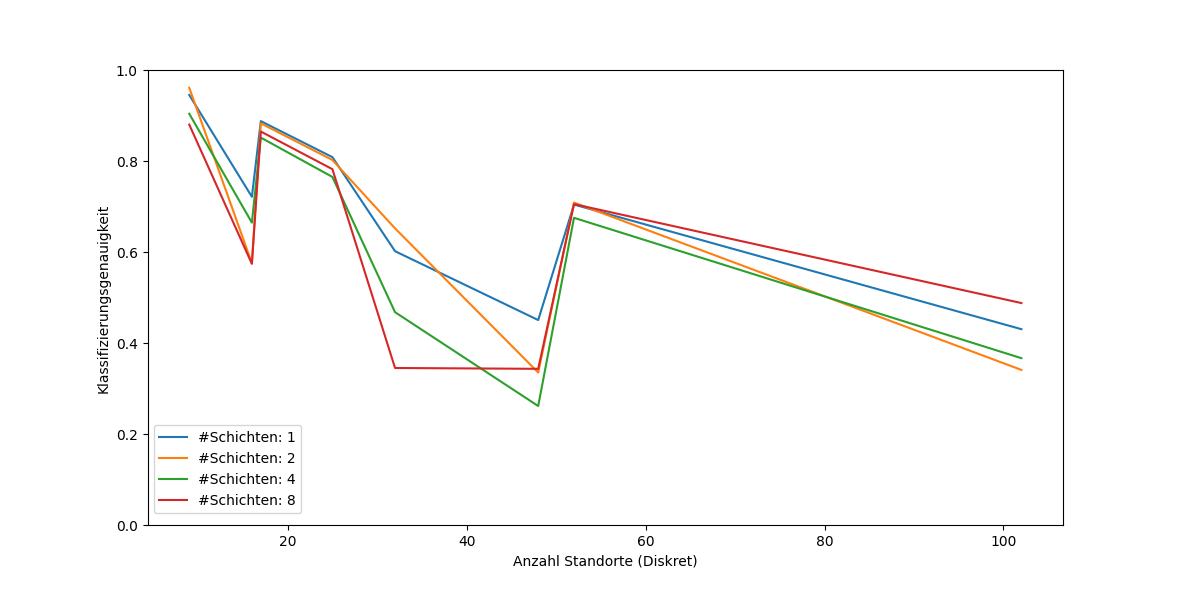
\includegraphics[width=\linewidth]{images/multiple_best_by_group_knn_layers_acc_5_cont.png}
    \caption{Klassifizierungsgenauigkeiten $P(B\leq5)_{\text{cont}}$ von FFNNs mit 32 Neuronen pro verdeckte Schicht über Standortkomplexitäten.}
    \label{fig:multiple_best_by_group_knn_layers_acc_5_cont}
\end{figure}

\begin{figure}[h!]
    \centering
    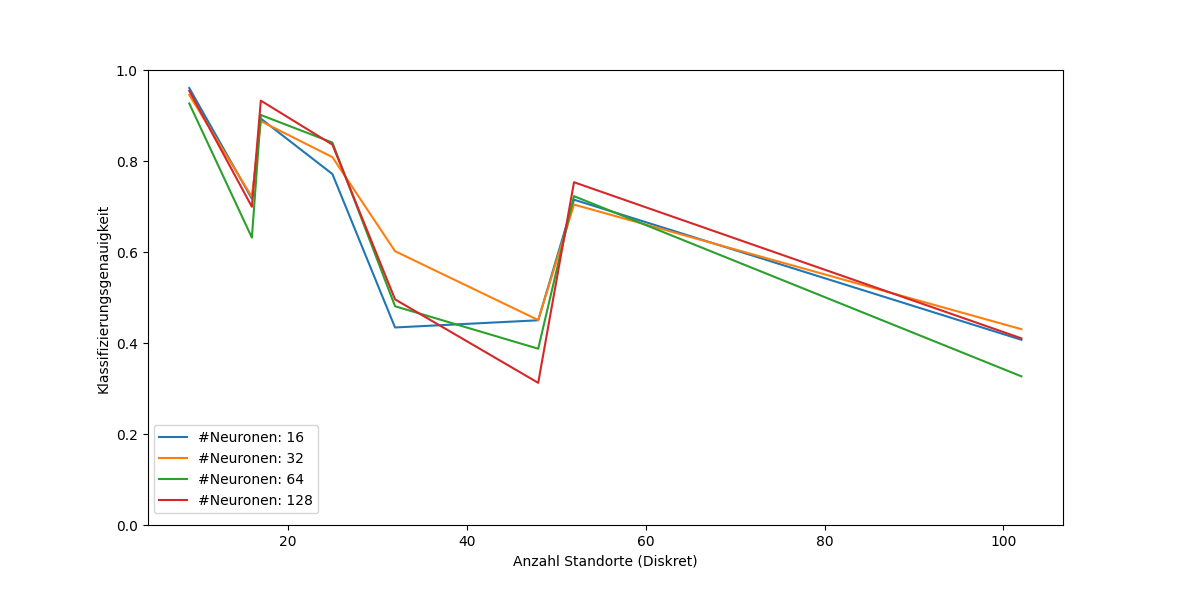
\includegraphics[width=\linewidth]{images/multiple_best_by_group_knn_neurons_acc_5_cont.png}
    \caption{Klassifizierungsgenauigkeiten $P(B\leq5)_{\text{cont}}$ von FFNNs mit einer verdeckte Schicht über Standortkomplexitäten.}
    \label{fig:multiple_best_by_group_knn_neurons_acc_5_cont}
\end{figure}

\begin{figure}[h!]
    \centering
    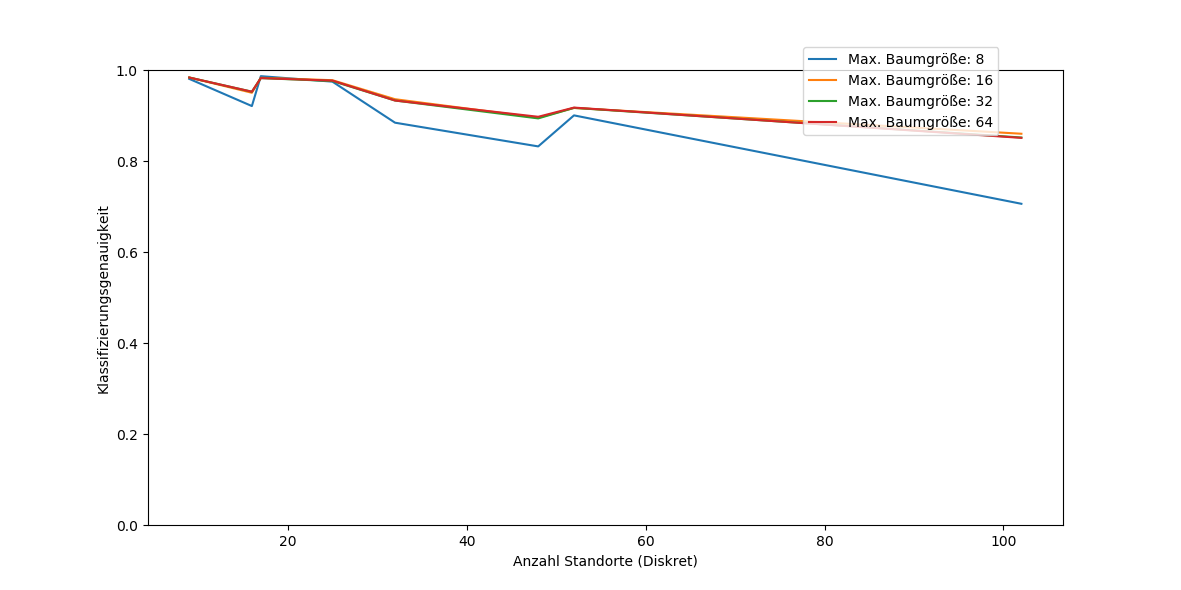
\includegraphics[width=\linewidth]{images/multiple_best_by_group_dt_max_depth_acc_5.png}
    \caption{Klassifizierungsgenauigkeiten $P(B\leq5)$ von Entscheidungswäldern ohne Rückwärtskante mit einer Waldgröße von 16 über Standortkomplexitäten.}
    \label{fig:multiple_best_by_group_dt_max_depth_acc_5}
\end{figure}

\begin{figure}[h!]
    \centering
    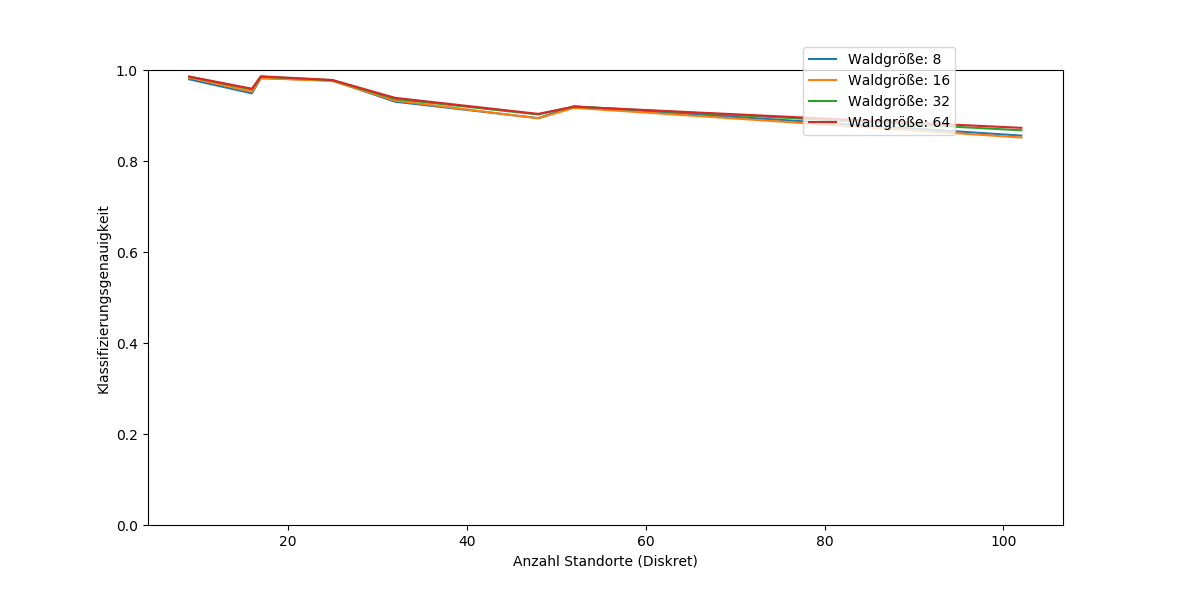
\includegraphics[width=\linewidth]{images/multiple_best_by_group_dt_trees_acc_5.png}
    \caption{Klassifizierungsgenauigkeiten $P(B\leq5)$ von Entscheidungswäldern ohne Rückwärtskante mit einer maximalen Baumhöhe von 32 über Standortkomplexitäten.}
    \label{fig:multiple_best_by_group_dt_trees_acc_5}
\end{figure}

\begin{figure}[h!]
    \centering
    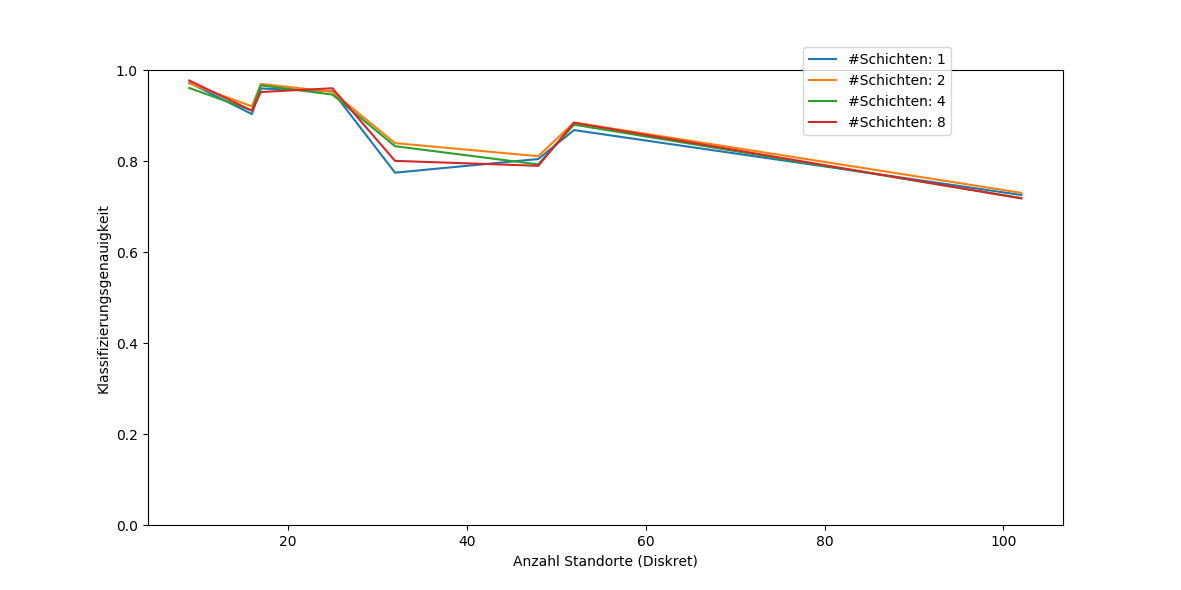
\includegraphics[width=\linewidth]{images/multiple_best_by_group_knn_layers_acc_5.png}
    \caption{Klassifizierungsgenauigkeiten $P(B\leq5)$ von FFNNs ohne Rückwärtskante mit 32 Neuronen pro verdeckte Schicht über Standortkomplexitäten.}
    \label{fig:multiple_best_by_group_knn_layers_acc_5}
\end{figure}

\begin{figure}[h!]
    \centering
    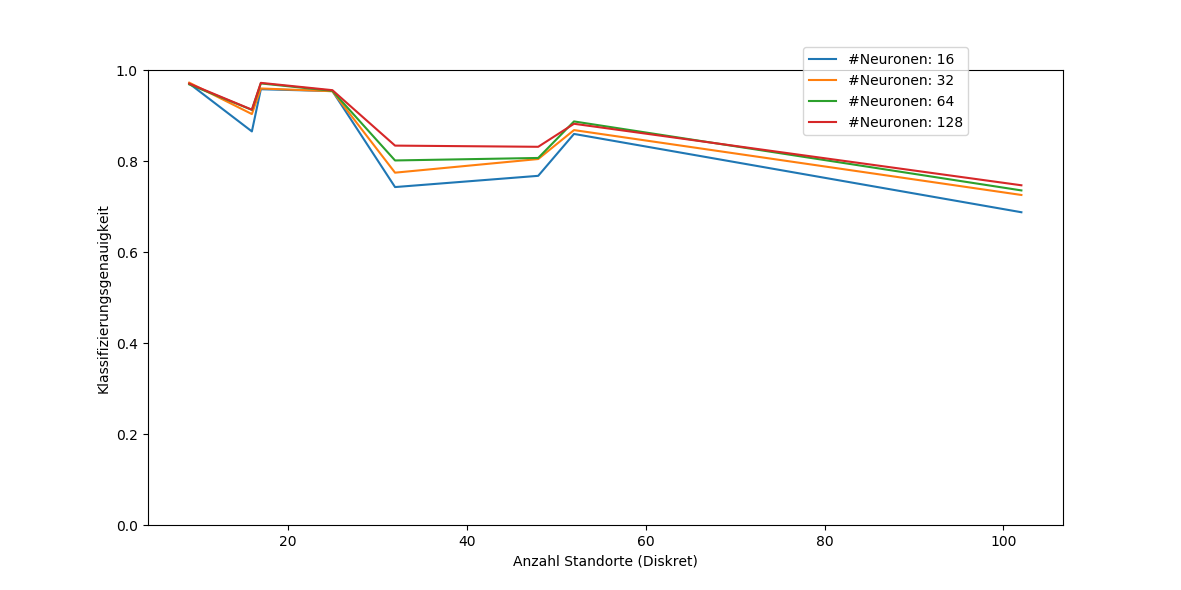
\includegraphics[width=\linewidth]{images/multiple_best_by_group_knn_neurons_acc_5.png}
    \caption{Klassifizierungsgenauigkeiten $P(B\leq5)$ von FFNNs ohne Rückwärtskante mit einer verdeckte Schicht über Standortkomplexitäten.}
    \label{fig:multiple_best_by_group_knn_neurons_acc_5}
\end{figure}

\begin{figure}[h!]
    \centering
    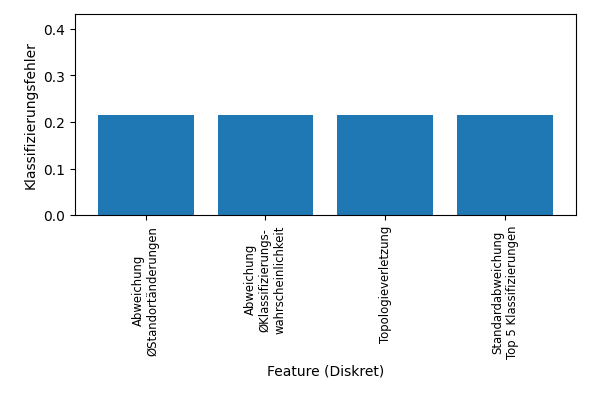
\includegraphics[width=\linewidth]{images/fi_knn_anomaly.png}
    \caption{Permutationswichtigkeit eines FFNNs zur Anomalieerkennung.}
    \label{fig:fi_knn_anomaly}
\end{figure}